\documentclass{beamer}

\usepackage[utf8]{inputenc}
\usepackage{hyperref}

\usetheme{Berkeley}
\beamertemplatenavigationsymbolsempty
\setbeamertemplate{headline}{}
 
\title{Highlighting in FoodChain-Lab}
\date{}
 
\begin{document}
\maketitle

\section{Tasks}
\begin{frame}
	\begin{itemize}
		\item Open the following workflow: \url{https://github.com/SiLeBAT/BfROpenLabResources/raw/master/GitHubPages/workflows/Small_Example.zip}.
		\item Change the color of \textbf{Outbreak} stations in the \textbf{Tracing View} from red to turquoise.
		\item Add the label "node" to each station.
	\end{itemize}
\end{frame}
 
\section{1}
\begin{frame}
	\begin{center}
  		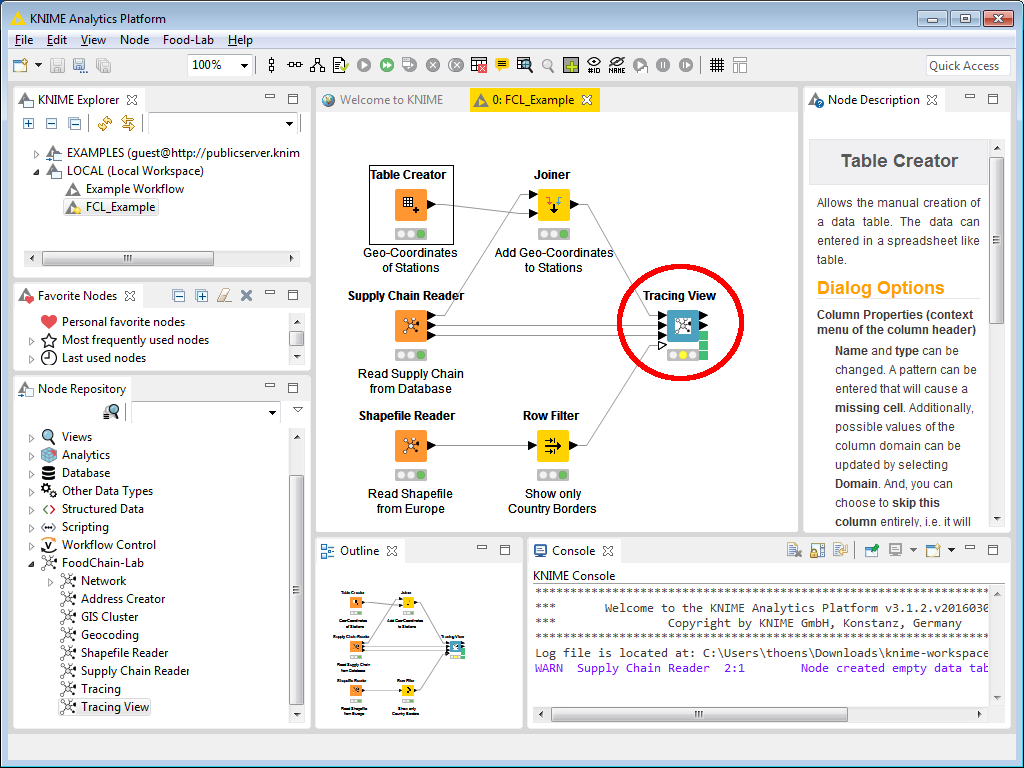
\includegraphics[height=0.6\textheight]{1.png}
	\end{center}
	\begin{itemize}
		\item Import the Small Example Workflow from \url{https://github.com/SiLeBAT/BfROpenLabResources/raw/master/GitHubPages/workflows/Small_Example.zip}.
		\item Open the \textbf{Tracing View} by double-clicking on it.
	\end{itemize}
\end{frame}

\section{2}
\begin{frame}
	\begin{center}
  		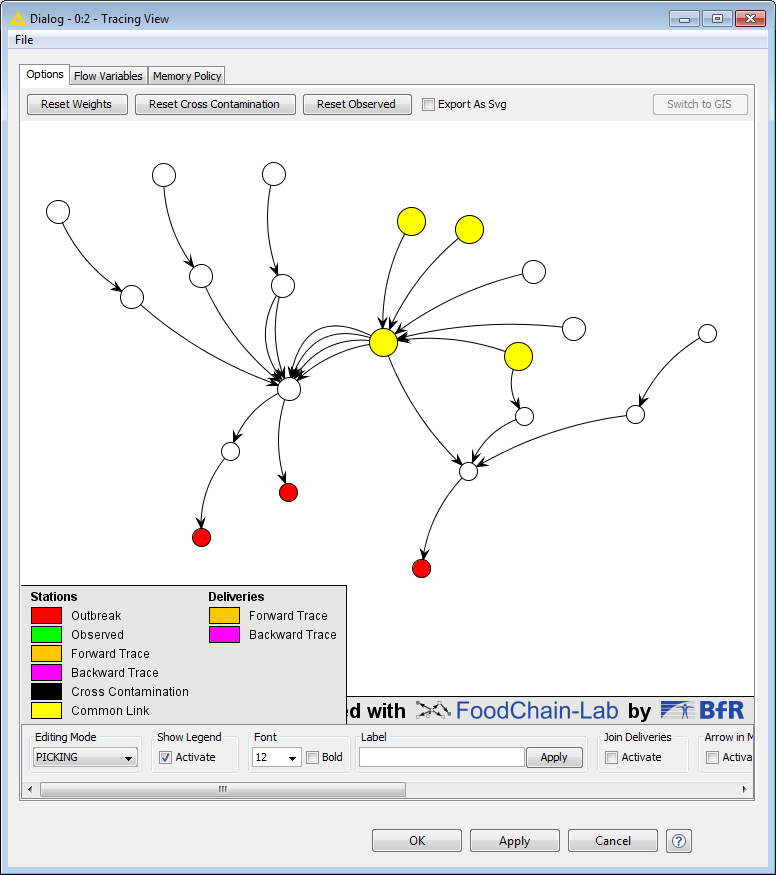
\includegraphics[height=0.6\textheight]{2.png}
	\end{center}
	\begin{itemize}
		\item Here you can see a small delivery graph with three outbreak locations (red stations) in the lower part.
	\end{itemize}
\end{frame}

\section{3}
\begin{frame}
	\begin{center}
  		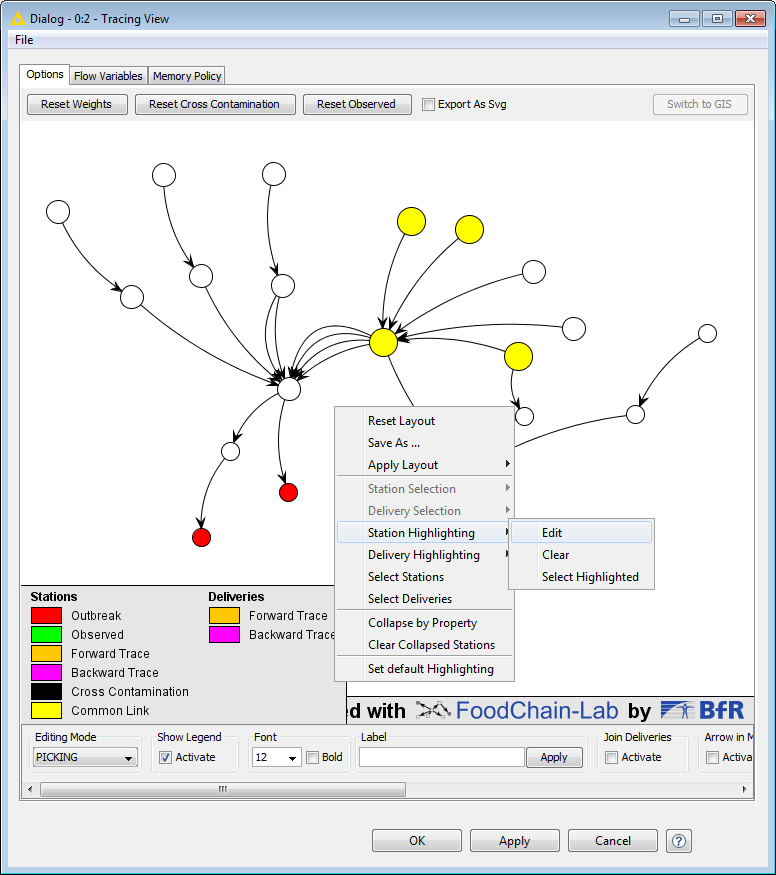
\includegraphics[height=0.6\textheight]{3.png}
	\end{center}
	\begin{itemize}
		\item Let's now change the color of the outbreak stations.
		\item Right click in the graph and select \textbf{Station Highlighting $>$ Edit}.
	\end{itemize}
\end{frame}

\section{4}
\begin{frame}
	\begin{center}
  		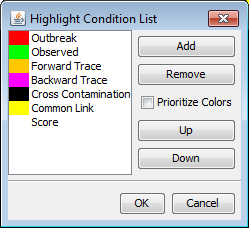
\includegraphics[height=0.6\textheight]{4.png}
	\end{center}
	\begin{itemize}
		\item A dialog with all defined highlighting conditions will pop up.
		\item Double click on the \textbf{Outbreak} condition to edit it.
	\end{itemize}
\end{frame}

\section{5}
\begin{frame}
	\begin{center}
  		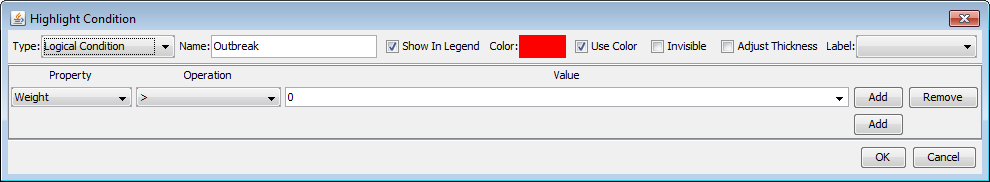
\includegraphics[width=0.9\textwidth]{5.png}
	\end{center}
	\begin{itemize}
		\item A new dialog for editing the outbreak condition will pop up.
		\item In this dialog you can also change what stations the highlighting should be applied to.
		\item Currently it is applied on all station with "Weight" $>$ 0. You can add other expressions by pressing the \textbf{Add} button on the right. These expressions can be combined via "And" or "Or".
		\item To edit the color click red square next to \textbf{Color}.
	\end{itemize}
\end{frame}

\section{6}
\begin{frame}
	\begin{center}
  		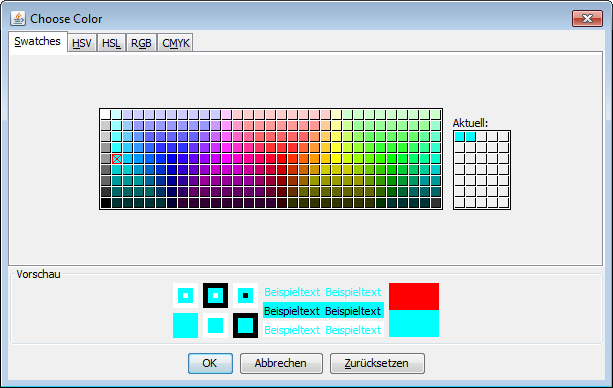
\includegraphics[height=0.6\textheight]{6.png}
	\end{center}
	\begin{itemize}
		\item In the color chooser dialog select turquoise and press \textbf{OK}.
	\end{itemize}
\end{frame}

\section{7}
\begin{frame}
	\begin{center}
  		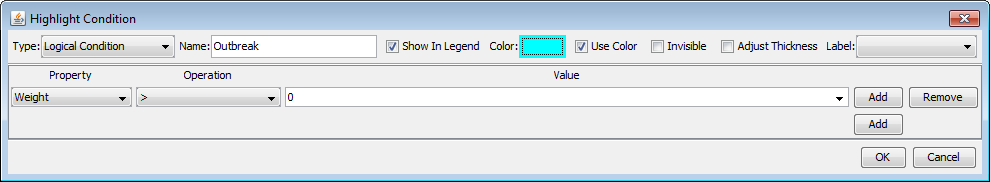
\includegraphics[width=0.9\textwidth]{7.png}
	\end{center}
	\begin{itemize}
		\item The square next to \textbf{Color} should be turquoise now.
		\item Press \textbf{OK}.
	\end{itemize}
\end{frame}

\section{8}
\begin{frame}
	\begin{center}
  		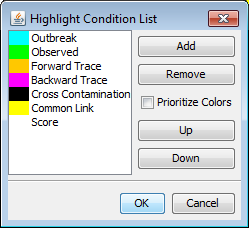
\includegraphics[height=0.6\textheight]{8.png}
	\end{center}
	\begin{itemize}
		\item In the dialog showing all highlighting conditions press \textbf{OK} to apply your changes.
	\end{itemize}
\end{frame}

\section{9}
\begin{frame}
	\begin{center}
  		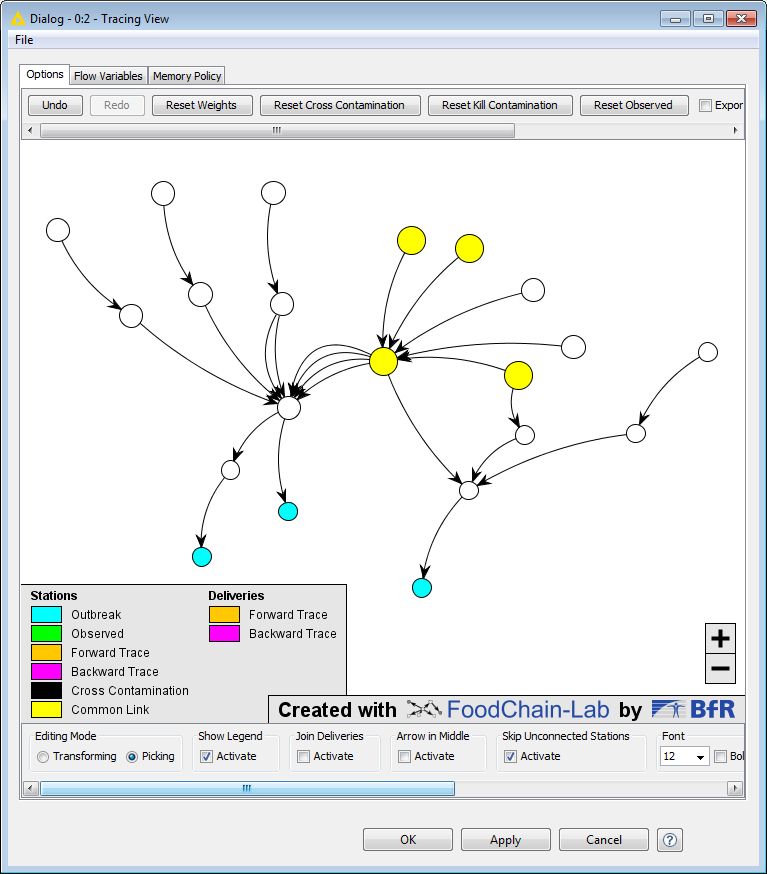
\includegraphics[height=0.6\textheight]{9.png}
	\end{center}
	\begin{itemize}
		\item The outbreak stations in the delivery graph should now be turquoise.
	\end{itemize}
\end{frame}

\section{10}
\begin{frame}
	\begin{center}
  		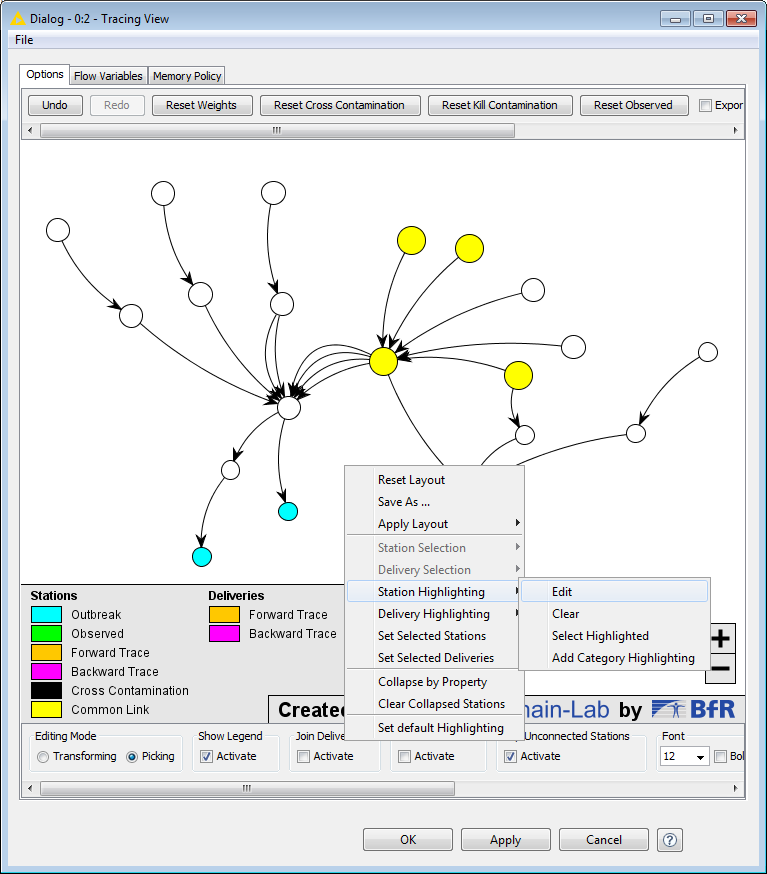
\includegraphics[height=0.6\textheight]{10.png}
	\end{center}
	\begin{itemize}
		\item Now we want to add labels to all stations in the graph.
		\item Right click in the graph and select \textbf{Station Highlighting $>$ Edit}.
	\end{itemize}
\end{frame}

\section{11}
\begin{frame}
	\begin{center}
  		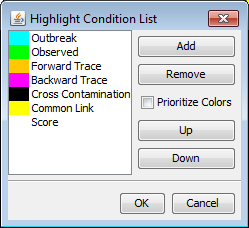
\includegraphics[height=0.6\textheight]{11.png}
	\end{center}
	\begin{itemize}
		\item We add the labelling as a new highlight condition.
		\item Press \textbf{Add} to add a new condition.
	\end{itemize}
\end{frame}

\section{12}
\begin{frame}
	\begin{center}
  		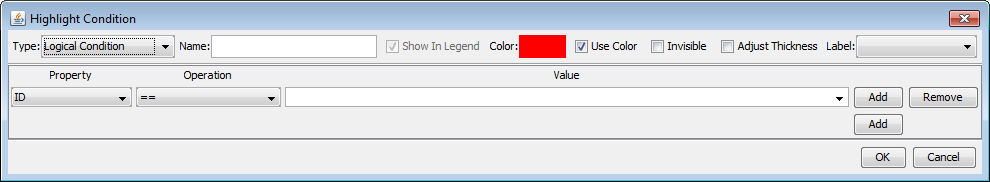
\includegraphics[width=0.9\textwidth]{12.png}
	\end{center}
	\begin{itemize}
		\item Add dialog will show up where you can configure the desired highlight condition.		
	\end{itemize}
\end{frame}

\section{13}
\begin{frame}
	\begin{center}
  		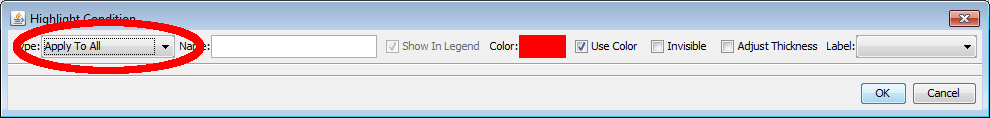
\includegraphics[width=0.9\textwidth]{13.png}
	\end{center}
	\begin{itemize}
		\item Since we want to use labels for all stations, select the \textbf{Type} "Apply To All".
	\end{itemize}
\end{frame}

\section{14}
\begin{frame}
	\begin{center}
  		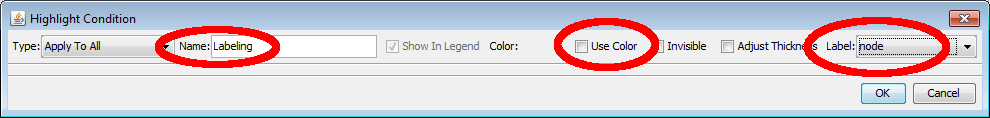
\includegraphics[width=0.9\textwidth]{14.png}
	\end{center}
	\begin{itemize}
		\item Set the \textbf{Name} to "Labelling" (just for documentation).
		\item Uncheck \textbf{Use Color}, since we just want to create labels with coloring.
		\item Set the \textbf{Label} to "node", since that is the column with station names.
		\item Press \textbf{OK} to create the highlight condition.
	\end{itemize}
\end{frame}

\section{15}
\begin{frame}
	\begin{center}
  		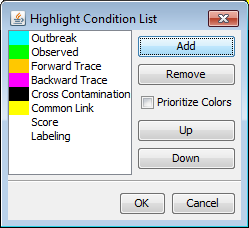
\includegraphics[height=0.6\textheight]{15.png}
	\end{center}
	\begin{itemize}
		\item In the dialog with all highlight conditions you should now see a new condition "Labelling".
		\item Press \textbf{OK} to apply the changes.
	\end{itemize}
\end{frame}

\section{16}
\begin{frame}
	\begin{center}
  		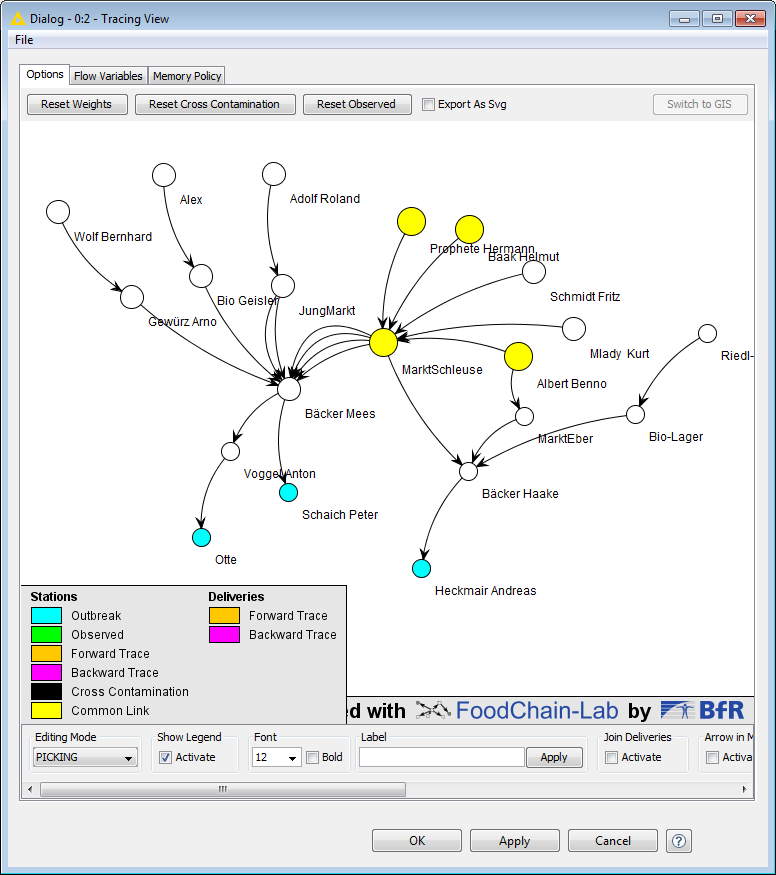
\includegraphics[height=0.6\textheight]{16.png}
	\end{center}
	\begin{itemize}
		\item In the delivery graph there is now a label next to each station.
	\end{itemize}
\end{frame}

\section{17}
\begin{frame}
	\begin{center}
  		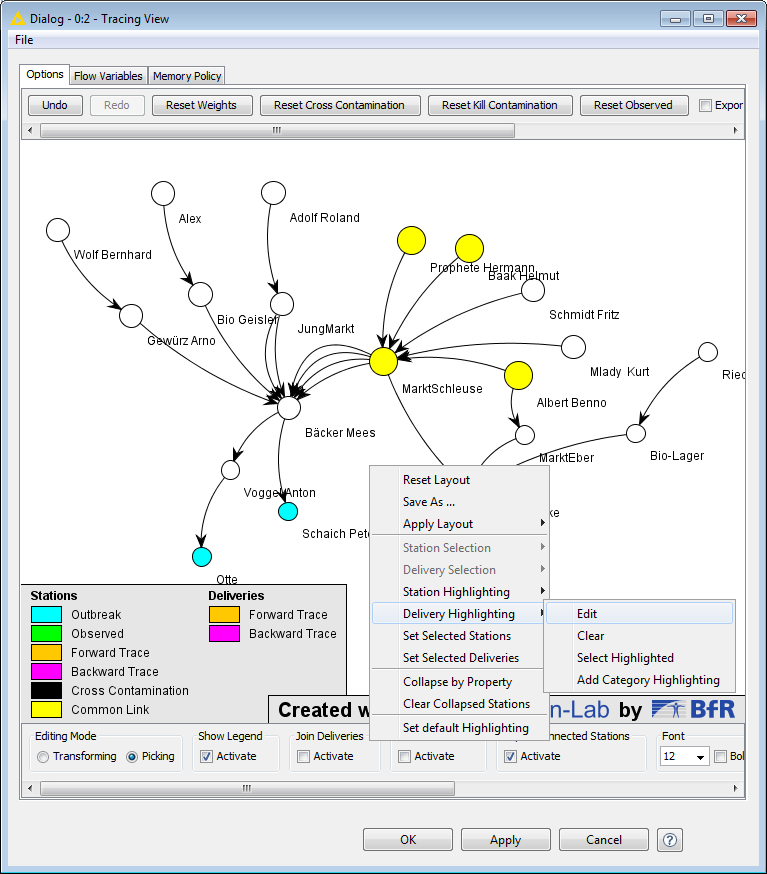
\includegraphics[height=0.6\textheight]{17.png}
	\end{center}
	\begin{itemize}
		\item FoodChain-Lab also allows to color or label deliveries the same way.
		\item To open the dialog for editing delivery highlight conditions right click in the graph and select \textbf{Delivery Highlighting $>$ Edit}.
	\end{itemize}
\end{frame}

\end{document}